% questions.tex —— 1982 年·全国卷（文科） · 题目内容片段（无答案）
% 由 tools/generate_projects.py 依来源总账自 1982/1982_数学真题_文_试题.md 生成，勿手改（改源 MD 后重跑）


\begin{gktip}
\textbf{来源说明}：本卷为 1982 年全国统一命题的\textbf{文科数学}卷（同年另有独立的理科卷，两份试卷题目不同），单页（原卷页码第 20 页），全卷共 9 题。题面不含答案（答案由本库独立推导）。原卷按左、中、右三栏分栏排版，本文按题号 1—9 顺序转录，题面文字未作改动。

\textbf{题面说明}：第 1、3 题为填表题，原卷表中“使函数有意义的 $x$ 的实数范围”“曲线名称”“图形”三列留空待填，本文照原卷保留空列。第 5、9 题依原卷配图重绘为 TikZ 矢量图。

\textbf{源注}：第 9 题原卷不等号印作“$\geqslant$”，本文统一转写为 $\ge$（与同期各卷一致）；该题“$B_1A_1\parallel BA$”“$B_2A_2\parallel BA$”中的平行号在纯文本提取时会丢失，本文按页面图像转录。
\end{gktip}

\begin{question}
\gkti{1}填表：

\begin{center}
\begin{tabular}{cll}
\toprule
 & 函数 & 使函数有意义的 $x$ 的实数范围 \\
\midrule
1 & $y=\sqrt{-x^2}$ &  \\
2 & $y=\sqrt{(-x)^2}$ &  \\
3 & $y=10^{\lg x}$ &  \\
4 & $y=\lg 10^x$ &  \\
\bottomrule
\end{tabular}
\end{center}

\end{question}
\begin{question}
\gkti{2}求 $(-1+\mathrm i)^{20}$ 展开式中第 15 项的数值。

\end{question}
\begin{question}
\gkti{3}在平面直角坐标系内，表中的方程表示什么曲线？并画出它们的图形：

\begin{center}
\begin{tabular}{clll}
\toprule
 & 方程 & 曲线名称 & 图形 \\
\midrule
1 & $4x^2+y^2=4$ &  &  \\
2 & $x-3=0$ &  &  \\
\bottomrule
\end{tabular}
\end{center}

\end{question}
\begin{question}
\gkti{4}已知 $x-y=\dfrac12$，$x^2+y^2=1$，求 $x^2-y^2$ 的值。

\Needspace{0.4\textheight}
\end{question}
\begin{question}
\gkti{5}以墙为一边，用篱笆围成长方形的场地，并用平行于一边的篱笆隔开（如图）。已知篱笆的总长为定值 $L$，这块场地的长和宽各为多少时场地的面积最大？最大面积是多少？
\nopagebreak[4]
\begin{center}% 1982 年全国卷（文科）第 5 题：以墙为一边、用篱笆围长方形场地，并以平行于宽边的篱笆隔成两块；上沿为带砖缝与短刻线的墙，墙两端略长于场地，左块窄、右块宽（按源卷布局）
\begin{tikzpicture}[scale=1, line width=0.5pt,
  every node/.style={inner sep=1.5pt}]
  % 墙：上沿 y=4.00、下沿 y=3.60 两条水平线
  \draw (0,4.00) -- (8,4.00);
  \draw (0,3.60) -- (8,3.60);
  % 砖缝（两线之间）
  \foreach \x in {0.65,1.45,2.25,3.05,3.85,4.65,5.45,6.25,7.05,7.85} {
    \draw (\x,3.60) -- (\x,4.00);
  }
  % 上沿短刻线
  \foreach \x in {0.25,1.05,1.85,2.65,3.45,4.25,5.05,5.85,6.65,7.45} {
    \draw (\x,4.00) -- (\x,4.27);
  }
  % 下沿短刻线
  \foreach \x in {0.25,1.05,1.85,2.65,3.45,4.25,5.05,5.85,6.65,7.45} {
    \draw (\x,3.60) -- (\x,3.33);
  }
  % 场地：左篱、中隔篱（平行于两侧的篱笆）、右篱均上端接墙的下沿，另加下横篱
  \draw (1.00,3.60) -- (1.00,0.38);
  \draw (2.95,3.60) -- (2.95,0.38);
  \draw (6.90,3.60) -- (6.90,0.38);
  \draw (1.00,0.38) -- (6.90,0.38);
\end{tikzpicture}
\end{center}
\nopagebreak[4]
\end{question}
\begin{question}
\gkti{6}已知正方体 $ABCD\text{-}A_1B_1C_1D_1$ 的棱长为 $a$。

（1） 用平面 $A_1BC_1$ 截去一角后，求剩余部分的体积；

（2） 求 $A_1B$ 和 $B_1C$ 所成的角。

\end{question}
\begin{question}
\gkti{7}已知定点 $A$、$B$ 且 $AB=2a$，如果动点 $P$ 到点 $A$ 的距离和到点 $B$ 的距离之比为 $2:1$，求点 $P$ 的轨迹方程，并说明它表示什么曲线。

\end{question}
\begin{question}
\gkti{8}求 $\tan 9^\circ+\cot 117^\circ-\tan 243^\circ-\cot 351^\circ$ 的值。

\Needspace{0.4\textheight}
\end{question}
\begin{question}
\gkti{9}如图，已知 $\triangle AOB$ 中，$OA=b$，$OB=a$，$\angle AOB=\theta$（$a\ge b$，$\theta$ 是锐角）。作 $AB_1\perp OB$，$B_1A_1\parallel BA$；再作 $A_1B_2\perp OB$，$B_2A_2\parallel BA$；如此无限连续作下去。设 $\triangle ABB_1$，$\triangle A_1B_1B_2$，$\cdots$ 的面积分别为 $S_1$，$S_2$，$\cdots$，求无穷数列 $S_1$，$S_2$，$\cdots$ 的和。
\nopagebreak[4]
\begin{center}% 1982 年全国卷（文科）第 9 题：△AOB 中作 AB₁⊥OB、B₁A₁∥BA，再作 A₁B₂⊥OB、B₂A₂∥BA，如此无限作下去；图中 OB 画成竖直线，故垂线 AB₁、A₁B₂、A₂B₃ 为水平线，阴影自下而上依次为 △ABB₁、△A₁B₁B₂、△A₂B₂B₃（按源卷布局）
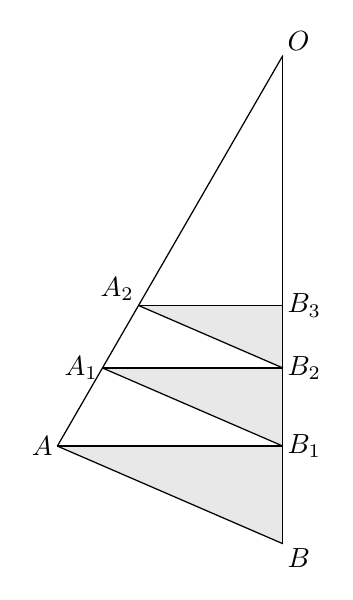
\begin{tikzpicture}[scale=0.62, line width=0.45pt,
  every node/.style={inner sep=1.5pt}]
  % OB 竖直（长 10），OA=b=9.238、∠AOB=θ=30°，公比 k=b·cosθ/a=0.8
  \coordinate (O)  at (0,10);
  \coordinate (B)  at (0,0);
  \coordinate (A)  at (-4.619,2.0);
  \coordinate (B1) at (0,2.0);
  \coordinate (A1) at (-3.695,3.6);
  \coordinate (B2) at (0,3.6);
  \coordinate (A2) at (-2.956,4.88);
  \coordinate (B3) at (0,4.88);
  % 阴影三角形（自下而上依次为 S₁、S₂、S₃）
  \fill[gray!18] (A) -- (B) -- (B1) -- cycle;
  \fill[gray!18] (A1) -- (B1) -- (B2) -- cycle;
  \fill[gray!18] (A2) -- (B2) -- (B3) -- cycle;
  % 各边
  \draw (O) -- (B);
  \draw (O) -- (A);
  \draw (A) -- (B);
  \draw (A) -- (B1);
  \draw (A1) -- (B1);
  \draw (A1) -- (B2);
  \draw (A2) -- (B2);
  \draw (A2) -- (B3);
  % 顶点标注
  \node[anchor=south west] at (O)  {$O$};
  \node[anchor=north west] at (B)  {$B$};
  \node[anchor=east]       at (A)  {$A$};
  \node[anchor=east]       at (A1) {$A_1$};
  \node[anchor=south east] at (A2) {$A_2$};
  \node[anchor=west]       at (B1) {$B_1$};
  \node[anchor=west]       at (B2) {$B_2$};
  \node[anchor=west]       at (B3) {$B_3$};
\end{tikzpicture}
\end{center}
\nopagebreak[4]

\end{question}